%%%%%%%%%%%%%%%%%%%%%%%%%%%%%%%%%%%%%%%%%
% Wenneker Assignment
% LaTeX Template
% Version 2.0 (12/1/2019)
%
% This template originates from:
% http://www.LaTeXTemplates.com
%
% Authors:
% Vel (vel@LaTeXTemplates.com)
% Frits Wenneker
%
% License:
% CC BY-NC-SA 3.0 (http://creativecommons.org/licenses/by-nc-sa/3.0/)
% 
%%%%%%%%%%%%%%%%%%%%%%%%%%%%%%%%%%%%%%%%%

%----------------------------------------------------------------------------------------
%	PACKAGES AND OTHER DOCUMENT CONFIGURATIONS
%----------------------------------------------------------------------------------------
\DeclareUnicodeCharacter{2212}{-}
\documentclass[11pt]{scrartcl} % Font size

%%%%%%%%%%%%%%%%%%%%%%%%%%%%%%%%%%%%%%%%%
% Wenneker Assignment
% Structure Specification File
% Version 2.0 (12/1/2019)
%
% This template originates from:
% http://www.LaTeXTemplates.com
%
% Authors:
% Vel (vel@LaTeXTemplates.com)
% Frits Wenneker
%
% License:
% CC BY-NC-SA 3.0 (http://creativecommons.org/licenses/by-nc-sa/3.0/)
% 
%%%%%%%%%%%%%%%%%%%%%%%%%%%%%%%%%%%%%%%%%

%----------------------------------------------------------------------------------------
%	PACKAGES AND OTHER DOCUMENT CONFIGURATIONS
%----------------------------------------------------------------------------------------
\usepackage{listings}
\usepackage{xcolor}

\definecolor{codegreen}{rgb}{0,0.6,0}
\definecolor{codegray}{rgb}{0.5,0.5,0.5}
\definecolor{codepurple}{rgb}{0.58,0,0.82}
\definecolor{backcolour}{rgb}{0.95,0.95,0.92}

\lstdefinestyle{mystyle}{
    backgroundcolor=\color{backcolour},   
    commentstyle=\color{codegreen},
    keywordstyle=\color{magenta},
    numberstyle=\tiny\color{codegray},
    stringstyle=\color{codepurple},
    basicstyle=\ttfamily\footnotesize,
    breakatwhitespace=false,         
    breaklines=true,                 
    captionpos=b,                    
    keepspaces=true,                 
    numbers=left,                    
    numbersep=5pt,                  
    showspaces=false,                
    showstringspaces=false,
    showtabs=false,                  
    tabsize=2
}

\lstset{style=mystyle}
\usepackage{amsmath, amsfonts, amsthm} % Math packages

\usepackage{listings} % Code listings, with syntax highlighting

\usepackage[english]{babel} % English language hyphenation

\usepackage{graphicx} % Required for inserting images
\graphicspath{{Figures/}{./}} % Specifies where to look for included images (trailing slash required)

\usepackage{booktabs} % Required for better horizontal rules in tables

\numberwithin{equation}{section} % Number equations within sections (i.e. 1.1, 1.2, 2.1, 2.2 instead of 1, 2, 3, 4)
\numberwithin{figure}{section} % Number figures within sections (i.e. 1.1, 1.2, 2.1, 2.2 instead of 1, 2, 3, 4)
\numberwithin{table}{section} % Number tables within sections (i.e. 1.1, 1.2, 2.1, 2.2 instead of 1, 2, 3, 4)

\setlength\parindent{0pt} % Removes all indentation from paragraphs

\usepackage{enumitem} % Required for list customisation
\setlist{noitemsep} % No spacing between list items

%----------------------------------------------------------------------------------------
%	DOCUMENT MARGINS
%----------------------------------------------------------------------------------------

\usepackage{geometry} % Required for adjusting page dimensions and margins

\geometry{
	paper=a4paper, % Paper size, change to letterpaper for US letter size
	top=2.5cm, % Top margin
	bottom=3cm, % Bottom margin
	left=3cm, % Left margin
	right=3cm, % Right margin
	headheight=0.75cm, % Header height
	footskip=1.5cm, % Space from the bottom margin to the baseline of the footer
	headsep=0.75cm, % Space from the top margin to the baseline of the header
	%showframe, % Uncomment to show how the type block is set on the page
}

%----------------------------------------------------------------------------------------
%	FONTS
%----------------------------------------------------------------------------------------

\usepackage[utf8]{inputenc} % Required for inputting international characters
\usepackage[T1]{fontenc} % Use 8-bit encoding

\usepackage{fourier} % Use the Adobe Utopia font for the document

%----------------------------------------------------------------------------------------
%	SECTION TITLES
%----------------------------------------------------------------------------------------

\usepackage{sectsty} % Allows customising section commands

\sectionfont{\vspace{6pt}\centering\normalfont\scshape} % \section{} styling
\subsectionfont{\normalfont\bfseries} % \subsection{} styling
\subsubsectionfont{\normalfont\itshape} % \subsubsection{} styling
\paragraphfont{\normalfont\scshape} % \paragraph{} styling

%----------------------------------------------------------------------------------------
%	HEADERS AND FOOTERS
%----------------------------------------------------------------------------------------

\usepackage{scrlayer-scrpage} % Required for customising headers and footers

\ohead*{} % Right header
\ihead*{} % Left header
\chead*{} % Centre header

\ofoot*{} % Right footer
\ifoot*{} % Left footer
\cfoot*{\pagemark} % Centre footer
 % Include the file specifying the document structure and custom commands

%----------------------------------------------------------------------------------------
%	TITLE SECTION
%----------------------------------------------------------------------------------------

\title{	
	\normalfont\normalsize
	\textsc{\Huge Physics-1 Lab SM203P}\\ % Your university, school and/or department name(s)
	\vspace{25pt} % Whitespace
	\rule{\linewidth}{0.5pt}\\ % Thin top horizontal rule
	\vspace{20pt} % Whitespace
	{\huge Experiment 2: Experiments with simple and double pendulums with phase portraits}\\ % The assignment title
	\vspace{12pt} % Whitespace
	\rule{\linewidth}{2pt}\\ % Thick bottom horizontal rule
	\vspace{12pt} % Whitespace
}

\author{\Huge Group-16\\
\\
\LARGE Mayank Chadha(IMT2020045)\\
\\
\LARGE Anshul Jindal(IMT2020039)\\
\\
\LARGE Rahul Jain(IMT2020117)\\
\\
\LARGE Karanjit Saha(IMT2020003)\\
\\
\LARGE Chinmay Parekh(IMT2020069)\\
\\
\LARGE Shashank Shekhar(IMT2020112)} % Your name

\date{\normalsize\today} % Today's date (\today) or a custom date

\begin{document}

\maketitle % Print the title
%----------------------------------------------------------------------------------------
%	FIGURE EXAMPLE
%----------------------------------------------------------------------------------------

\begin{figure}[h] % [h] forces the figure to be output where it is defined in the code (it suppresses floating)
	\centering
	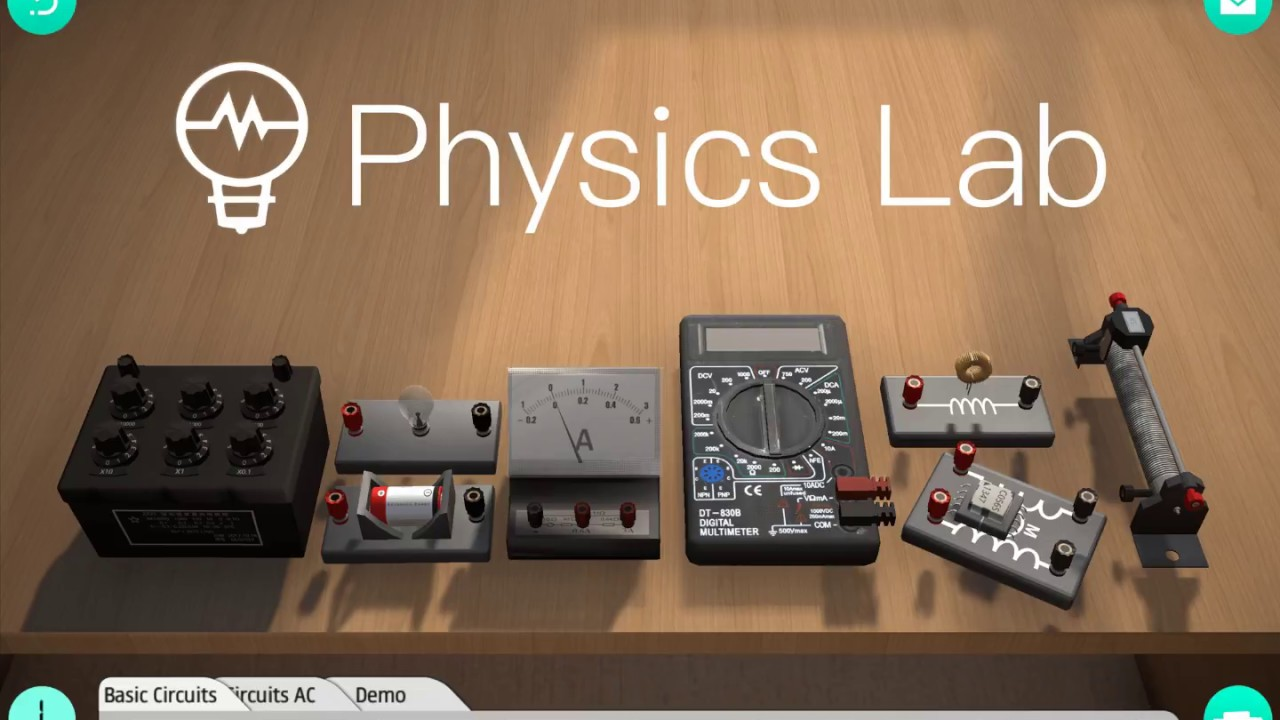
\includegraphics[width=\textwidth, height=5cm]{first.jpg} % Example image
	\caption{Physics lab.}
\end{figure}

%------------------------------------------------
\section{Aim of Experiment}
1. To study the equation $x_{n+1} =$ r$x_n$(1 − $x_n$) and to see how it varies with r.\par
2.  To plot “orbit diagram” or “bifurcation diagram”. \par
3. To calculate Feigenbaum constant.  \par




%----------------------------------------------------------------------------------------
%	TEXT EXAMPLE
%----------------------------------------------------------------------------------------

%------------------------------------------------
\section{Theory}


\subsection{Logistic Map}
Logistic map is basically a mathematical relation of degree 2 which resembles simple \textbf{non-linear} dynamical equations. We will build a population growth model using it. Maps stands with the terminology of discrete systems which can be describes as a set of difference equations.\par

Logistic map is written as:

\begin{equation}
X_{n+1}=r X_{n}\left(1-X_{n}\right)
\end{equation}

Where:\par
\textbf{$X_{n}$} - It is the  entity that represents ratio of existing population to the maximum possible population.\par
\textbf{r} - It is the intrinsic growth rate. It depends on how population is being modelled. \par
 
It can be easily observed that:
\begin{equation*}
0 \leq X_{n} \leq 1
\end{equation*}

And if we plot the graph between $X_{n+1}$ and $X_{n}$, we will get a parabola. It will be maximum when $X_{n}$ = $\frac{1}{2}$ which happens when r = $\frac{1}{4}$.

Thus we also get:
\begin{equation*}
0 \leq r \leq 4
\end{equation*}
 
 
 \subsubsection{Assumptions}
 1. Population after the end of the next generation is directly proportional to the population at the end of current generation.\\
 2. Rate of population growth is proportional to size of population.\\
 3. If population very large -> sources consumed, so next generation dies out.

\subsection{Bifurcation Diagram}
A bifurcation is an abrupt change in the qualitative behavior of a system. Bifurcation Diagram is also called \textbf{Orbital Diagram}. It is basically a plot between X and r (i.e we will increase r from 0 to 4 and observe for all X we get).

\subsection{Feigenbaum Constant}

It is defined as:
\begin{equation}
\delta=\lim _{n \rightarrow \infty} \frac{r_{n}-r_{n-1}}{r_{n+1}-r_{n}}
\end{equation}\par

The above mentioned result is approximately equal to 4.669.....
\section{Sources of Error}
\begin{enumerate}
	\item Air Resistance
	\item Old Tennis ball
	\item Rigged Meter Scale
	\item Inclined or Rough Surface
	\item The value of e may change with the height.
	\item Time taken during the collision will also contribute to the wrong calculation of e
	\item Phyphox mobile app uses various sensors present in a mobile phone, which may not give accurate results every time.
	\item Electric and magnetic fields may disturb the working of the sensors, due to which the results observed may not be completely accurate.
	\item Acoustic stopwatch of the Phyphox app also takes some time to stop the timer after hearing the sound of the collision.
	\item Random error.
\end{enumerate}
%----------------------------------------------------------------------------------------
%	EQUATION EXAMPLES
%----------------------------------------------------------------------------------------
\newpage

\section{Observation and Calculation}
\textbf{Q1} - Common Code for the group :\par
\underline{NOTE}: We take r as input.\par
\begin{lstlisting}[language=Python, caption= Code for plotting $X_n$ vs n graph for a given r]
import matplotlib.pyplot as plt
import numpy as np
n = []
x_limit=150
for i in range (x_limit):
    n.append(i)
y = []
y.append(0.1)
k = 0.1
r = float(input())
for i in range (x_limit-1):
    k = r * k * (1 - k)
    y.append(k)
plt.xlabel("n")
plt.ylabel("$X_n$")
plt.title("r="+str(r))
plt.plot(n, y)
plt.show() 
\end{lstlisting}
\newpage
\subsection{Mayank Chadha(IMT2020045)}
\textbf{Q2}.
\begin{figure}[h] % [h] forces the figure to be output where it is defined in the code (it suppresses floating)
	\centering
	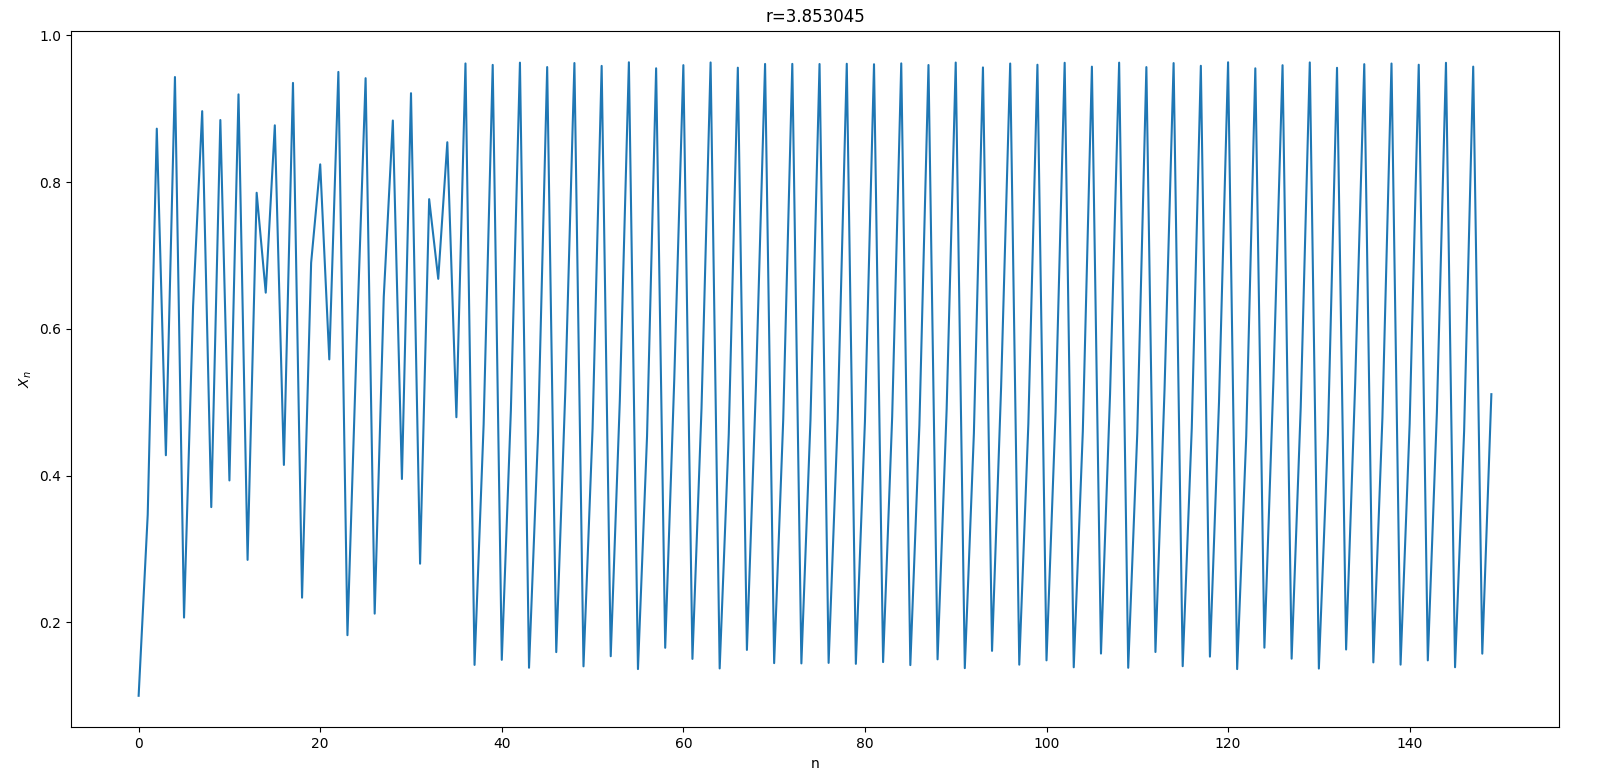
\includegraphics[width=12cm, height=8cm]{Mayank.png} % Example image
	\caption {Plot for $x_n$ vs n graph for r= 3.853045}
\end{figure}
\subsection{Anshul Jindal(IMT2020039)}
\textbf{Q2}.
\begin{figure}[h] % [h] forces the figure to be output where it is defined in the code (it suppresses floating)
	\centering
	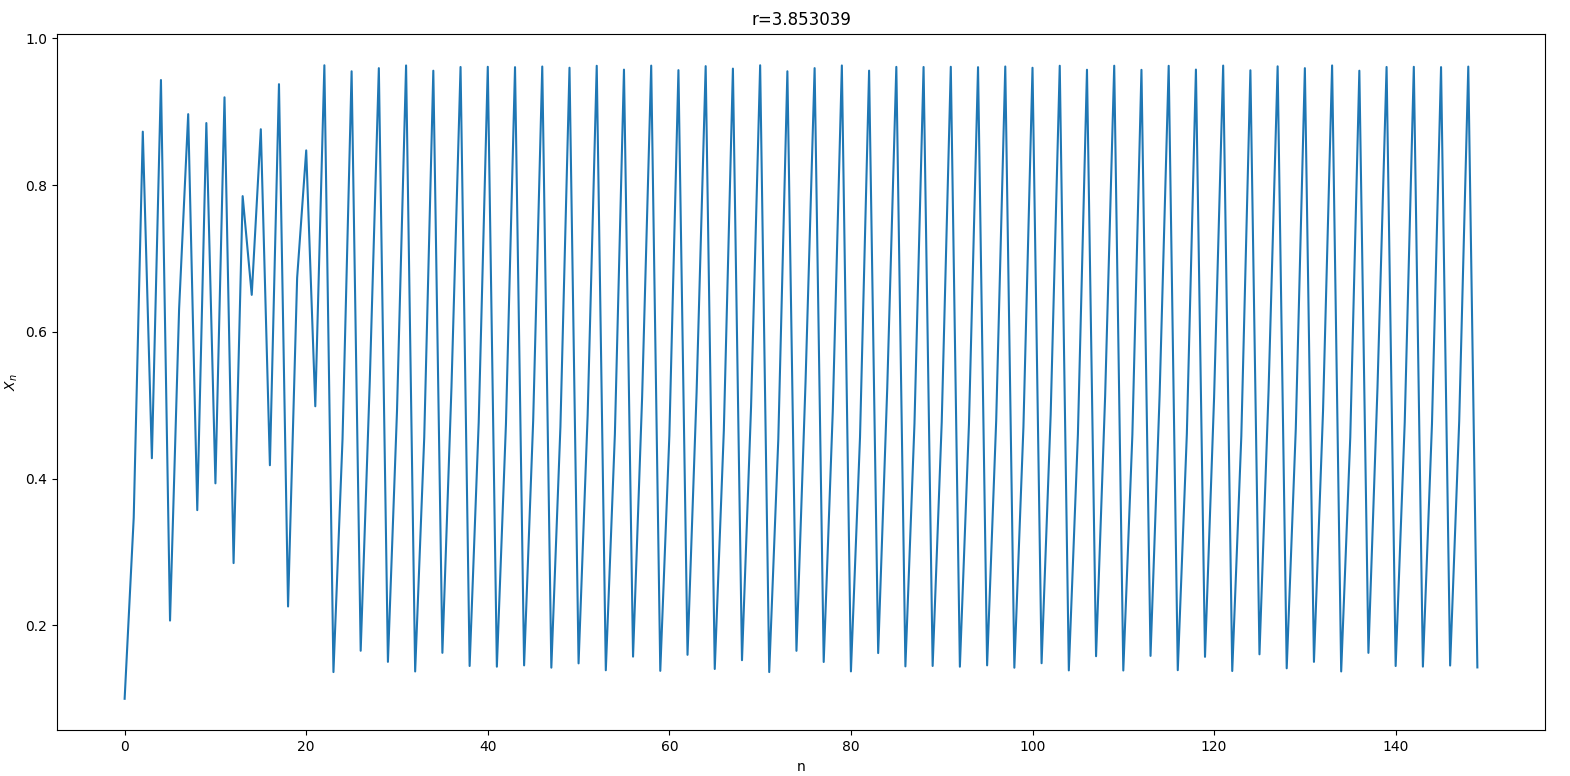
\includegraphics[width=12cm, height=8cm]{anshul_bsdk.png} % Example image
	\caption {Plot for $x_n$ vs n graph for r= 3.853039}
\end{figure}
\newpage
\subsection{Rahul Jain (IMT2020117)}
\textbf{Q2}.
\begin{figure}[h] % [h] forces the figure to be output where it is defined in the code (it suppresses floating)
	\centering
	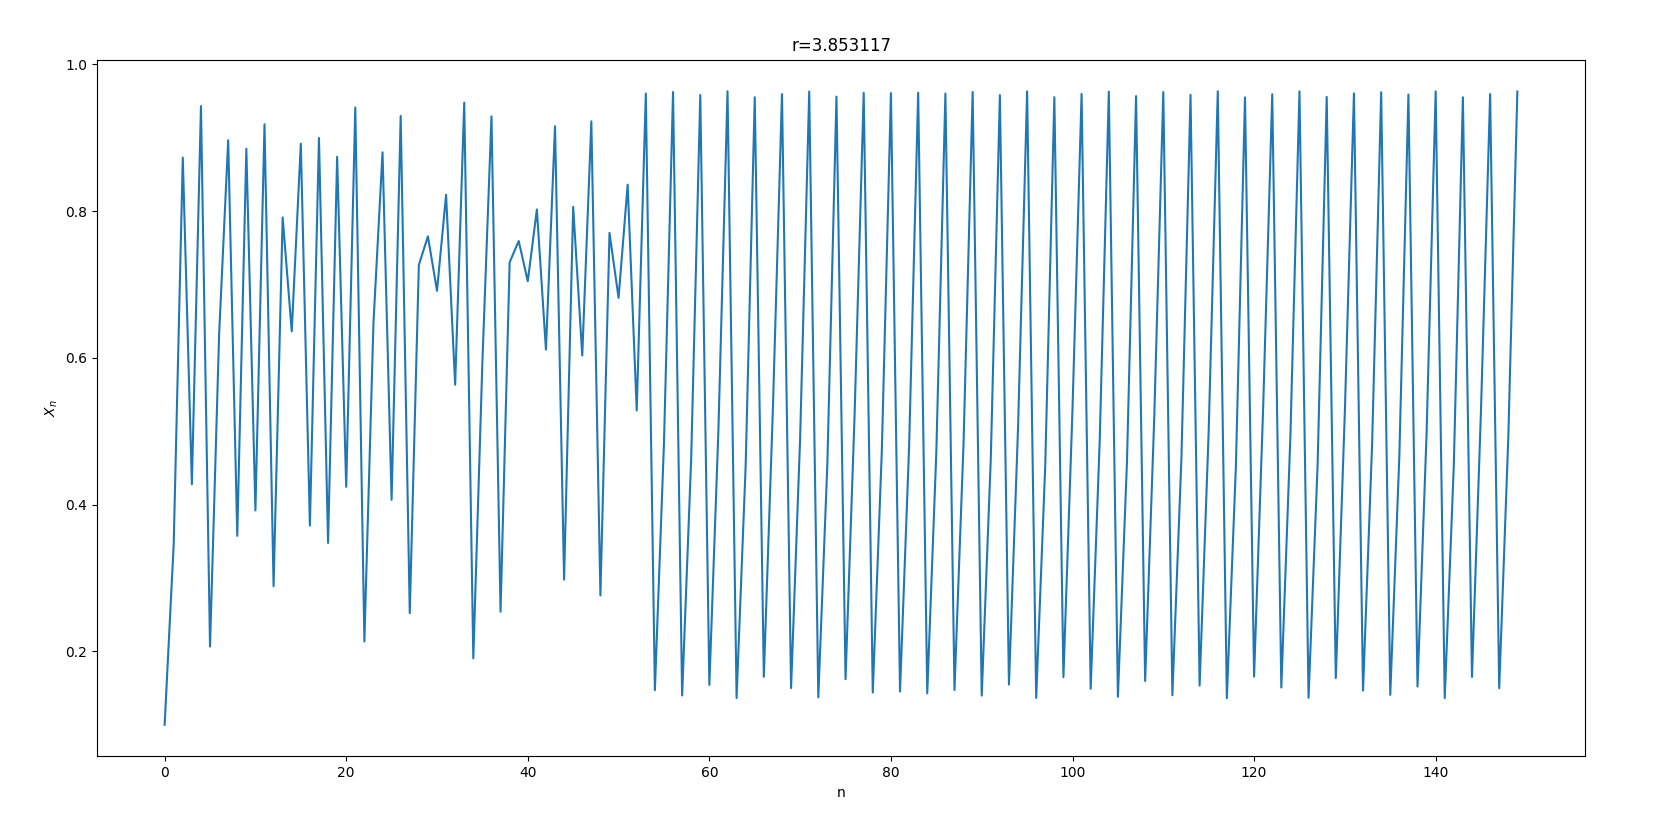
\includegraphics[width=12cm, height=8cm]{Rahul_singer.png} % Example image
	\caption {Plot for $x_n$ vs n graph for r= 3.853117}
\end{figure}
\subsection{Karanjit Saha (IMT2020003)}
\textbf{Q2}.
\begin{figure}[h] % [h] forces the figure to be output where it is defined in the code (it suppresses floating)
	\centering
	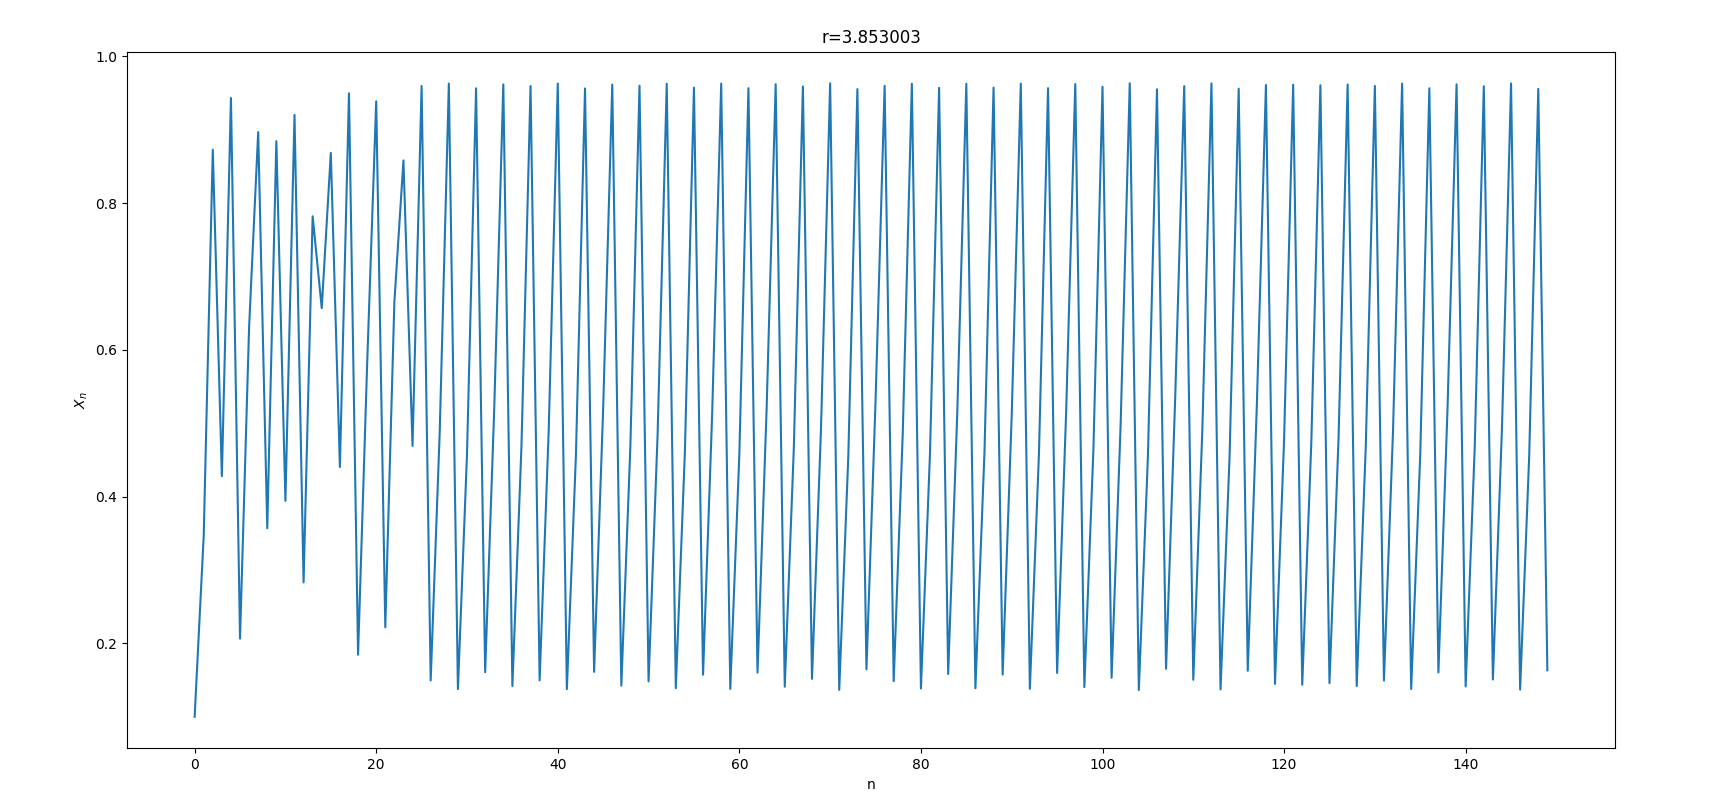
\includegraphics[width=12cm, height=8cm]{Karanjit.png} % Example image
	\caption {Plot for $x_n$ vs n graph for r= 3.853003}
\end{figure}
\newpage
\subsection{Chinmay Parekh (IMT2020069)}
\textbf{Q2}.
\begin{figure}[h] % [h] forces the figure to be output where it is defined in the code (it suppresses floating)
	\centering
	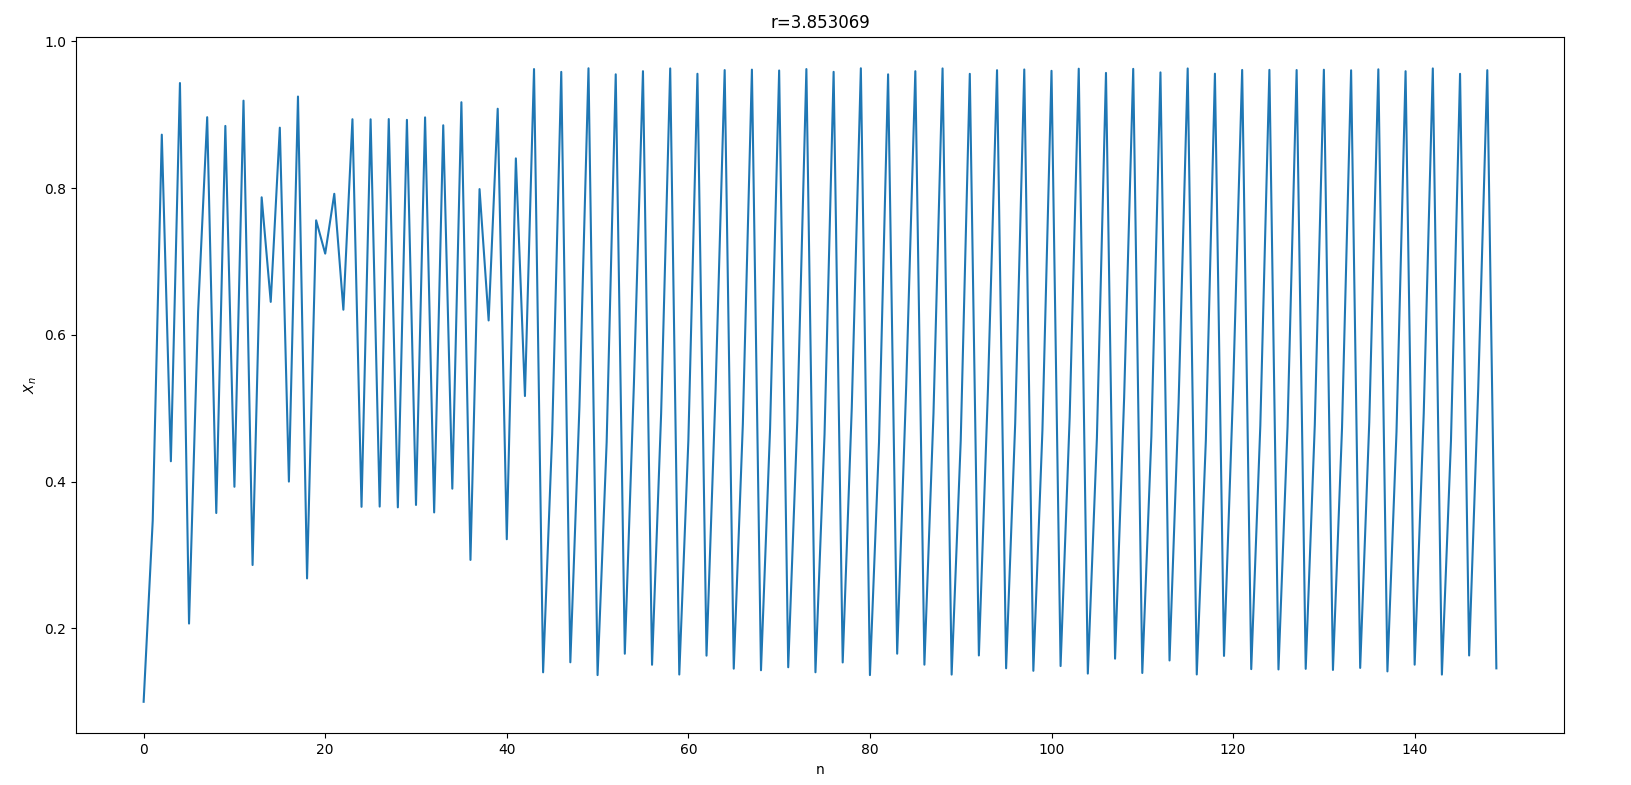
\includegraphics[width=12cm, height=8cm]{chinmay69.png} % Example image
	\caption {Plot for $x_n$ vs n graph for r= 3.853069}
\end{figure}
\subsection{Shashank Shekhar (IMT2020112)}
\textbf{Q2}.
\begin{figure}[h] % [h] forces the figure to be output where it is defined in the code (it suppresses floating)
	\centering
	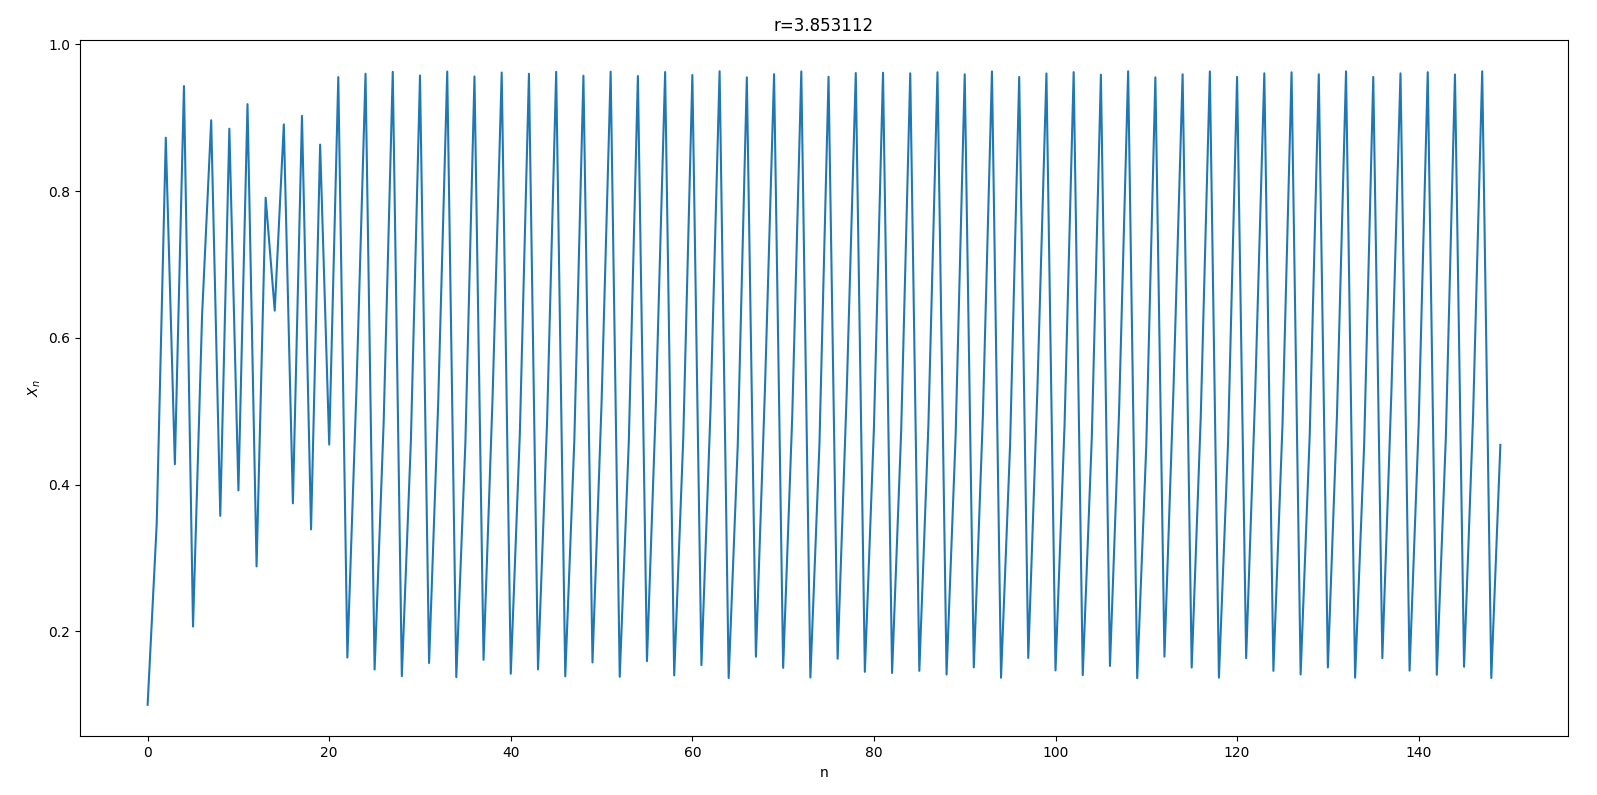
\includegraphics[width=12cm, height=8cm]{shashank.png} % Example image
	\caption {Plot for $x_n$ vs n graph for r= 3.853112}
\end{figure}
\newpage
\textbf{Q3(a)} - Common Code for the group :\par
\begin{lstlisting}[language=Python, caption= Bifurcation diagram]
import numpy as np
P=np.linspace(1,4,10000)
m=0.7
X = []
Y = []
for u in P:
    X.append(u)
    m = np.random.random()#starting with a random value of m.
    for n in range(1001):
      m=(u*m)*(1-m)
    for l in range(1051):
      m=(u*m)*(1-m)
    Y.append(m)
plt.xlabel("r")
plt.ylabel("x")
plt.plot(X, Y, ls='', marker=',')
plt.show()
\end{lstlisting}
\textbf{Q4} - Common Code for the group :\par
\begin{lstlisting}[language=Python, caption= Feigenbaum constants]
print ('Feigenbaum constant calculation:')
maximum_i = 16
maximum_j = 40
a1 = 1.0
a2 = 0.0
d1 = 3.2
print( 'iterations ', 'Feigenbaum constant')
for i in range(2, maximum_i):
    a = a1 + (a1 - a2) / d1
    for j in range(maximum_j):
        x = 0
        y = 0
        for k in range(2 ** i):
            y = 1 - 2 * y * x
            x = a - x * x    
        a = a - x / y
    d = (a1 - a2) / (a - a1)
    print ( i,"  ", d)
    d1 = d
    a2 = a1
    a1 = a
\end{lstlisting}
\end{document}